\documentclass[10pt]{beamer}

\usetheme{metropolis}
\usepackage{tcolorbox}


\usepackage{appendixnumberbeamer}

\usepackage{booktabs}
\usepackage[scale=2]{ccicons}

\usepackage{pgfplots}

\usepackage{xspace}
\newcommand{\themename}{\textbf{\textsc{metropolis}}\xspace}

%%%%%%%%%%%%%%%%%%%%%%%%%%%%%%%%%%%%%%%%%%%%%%
%
%		Thesis Settings
%		Custom settings
%
%		2011
%
%%%%%%%%%%%%%%%%%%%%%%%%%%%%%%%%%%%%%%%%%%%%%%

% %
% %   Use this file for your own custom packages, command-definitions, etc...
% %
% % 
% % Packages for references - cleverref must be last
% \usepackage{nameref}
% \usepackage{hyperref}
% \usepackage{cleveref}
% \usepackage[shortlabels]{enumitem}
% % Reduce spacing in bibliography
% \setlength{\bibsep}{0pt plus 0.3ex}
% % Allow equations to break between pages
% \allowdisplaybreaks
% % Penalty for widow and orphan
% \widowpenalty=9999
% \clubpenalty=9999
% %Penalty for relation and binary operation breaks in equations
% \relpenalty=9999
% \binoppenalty=9999


\usepackage{amsmath,amssymb,amsfonts, amsthm}
\usepackage{algorithmic}
\usepackage{graphicx}
\usepackage{textcomp}
\usepackage{xcolor}
\usepackage{hyperref}
\usepackage{import}
\usepackage{appendix}

\usepackage{pgfplots}
\usepackage[super]{nth}

\newcommand{\norm}[1]{\left\lVert#1\right\rVert}



%\newtheorem{result}{Result}[section]
%\newtheorem{lemma}{Lemma}[section]
%\newtheorem{definition}{Definition}[section]

\newcommand{\opL}{\mathcal L}
\newcommand{\opR}{\mathcal R}
\renewcommand{\Re}{\operatorname{Re}}
\renewcommand{\Im}{\operatorname{Im}}
\newcommand{\mean}[1]{\mathbb E#1}
\newcommand{\fmean}[1]{\langle #1 \rangle}
\newcommand{\cov}{\text{Cov}}
\newcommand{\var}{\text{Var}}
\newcommand{\trOp}[1]{(J \otimes \text{Tr}) \left[#1\right]}
\newcommand{\trace}[1]{\text{Tr}\left[#1\right]}
\newcommand{\Sp}{\text{Sp}}
\newcommand{\e}{\text {e}}
\newcommand{\dd}[1]{\mathrm{d}#1}
\newcommand{\traceLim}[2][.]{ \text{Tr}_{#1}\left[#2\right] }
\newcommand{\traceLimOp}[2][.]{ (J \otimes \text{Tr}_{#1})\left[#2\right] }

% Definitions of handy macros can go here

\newcommand{\dataset}{{\cal D}}
\newcommand{\fracpartial}[2]{\frac{\partial #1}{\partial  #2}}


\usepackage{subcaption}
\usepackage{graphicx}
\usepackage{amsfonts}
\usepackage{mathtools,amssymb}
\usepackage{graphicx}
\usepackage{float}
\usepackage{amsmath}
\usepackage{float}
\usepackage[super]{nth}
\usepackage{dsfont}
\usepackage{pgfplots}
\usepackage{adjustbox}
%\usepackage{enumitem,kantlipsum}

\usepackage{etoolbox}

\AtBeginEnvironment{subappendices}{%
\chapter*{Appendix}
\addcontentsline{toc}{chapter}{Appendices}
\counterwithin{figure}{section}
\counterwithin{table}{section}
}



\usepackage{tikz}
\usetikzlibrary{positioning}
\tikzset{%
  every neuron/.style={
    circle,
    draw,
    minimum size=1cm
  },
  neuron missing/.style={
    draw=none, 
    scale=2,
    text height=0.333cm,
    execute at begin node=\color{black}$\vdots$
  },
}


\renewcommand{\Re}{\operatorname{Re}}
\renewcommand{\Im}{\operatorname{Im}}
\newcommand{\Real}{\mathbb R}
\newcommand{\Complex}{\mathbb C}
\newcommand{\Integer}{\mathbb N}
\newcommand{\Normal}{\mathcal N}
\newcommand{\Matrix}{\mathcal M}


\newcommand{\MSEtrain}{\mathcal E_{\text{train}}}
\newcommand{\MSEtest}{ \mathcal E_{\text{gen}}}

\newcommand{\Etrain}[1][\lambda]{\mathcal E_{\text{train}}^#1}
\newcommand{\Egen}{\mathcal E_{\text{gen}}}

\newcommand{\barMSEtrain}{\bar{\mathcal E}_{\text{train}}}
\newcommand{\barMSEtest}{\bar{\mathcal E}_{\text{gen}}}


\newcommand{\activation}{\sigma}

\newcommand{\Zlin}{Z_{\text{lin}}}

\DeclareMathOperator\erf{erf}

\newcommand{\CORRECT}[2]{ \textcolor{red}{\st{#1}}\textcolor{blue}{#2} }

\newcommand{\simplenorm}[1]{\lVert#1\rVert}
\newcommand{\resolvent}[1]{\mathcal G^{#1}}



% Colors for the hyperref package
\definecolor{urlcolor}{rgb}{0,.145,.698}
\definecolor{linkcolor}{rgb}{.71,0.21,0.01}
\definecolor{citecolor}{rgb}{.12,.54,.11}

% Setup hyperref package
\hypersetup{
  breaklinks=true,  % so long urls are correctly broken across lines
  colorlinks=true,
  urlcolor=urlcolor,
  linkcolor=linkcolor,
  citecolor=citecolor,
}
% Slightly bigger margins than the latex defaults


\usepackage{fancyvrb}
\DefineVerbatimEnvironment{Verbatim}{Verbatim}{fontsize=\footnotesize}



\definecolor{grey}{rgb}{0.5, 0.5, 0.5}
\tikzset{%
  every neuron/.style={
    circle,
    draw,
    minimum size=0.3cm
  },
  neuron missing/.style={
    draw=none, 
    scale=2,
    text height=0.333cm,
    execute at begin node=\color{black}$\vdots$
  },
}
\usetikzlibrary{shadows.blur}
\usetikzlibrary{shapes.symbols}


\usepgfplotslibrary{dateplot}


\metroset{block=fill}
\useinnertheme[showtitle=false]{tcolorbox}

\title{Random matrix methods for high-dimensional\\ machine learning models}
\subtitle{A statistical limit theory for ML models}
\date{\today}
\author{Antoine Bodin}
\institute{EPFL}
% \titlegraphic{\hfill\includegraphics[height=1.5cm]{logo.pdf}}



\begin{document}

\maketitle

\begin{frame}{Table of contents}
  \setbeamertemplate{section in toc}[sections numbered]
  \tableofcontents[hideallsubsections]
\end{frame}

\section{Introduction \& motivational example}


\begin{frame}{Why Random Matrix theory needed?}
  \begin{alertblock}{}
    \textbf{Random matrices} are ubuquitous in machine learning theory.
    \textbf{But} using them is not always straightforward.
    \textbf{So} can we develop simple tools to analyze high-dimensional models involving random matrices?
  \end{alertblock}
  \emph{Example: linear-model}
  \begin{itemize}
    \item \textbf{Data:} $X \in \mathbb R^{n \times d}$ with $X_{ij} \sim \mathcal N(0, \frac{1}{d})$ ($n$ samples, $d$ features), 
    \item \textbf{Output:} $Y = X \beta^* + \xi$ with $\xi \sim \mathcal N(0, \sigma^2 I_n)$ and $ \frac{1}{d}\norm{\beta^*}^2 = r^2$
    \item \textbf{Model:} $\hat \beta = (X^T X + \lambda I_d)^{-1} X^T Y$ (ridge regression)
  \end{itemize}

  % Question
  
  \vspace{0.4cm}
  \begin{alertblock}{Generalization error}
    \emph{Averaging over new random data points ($x$ and $y=x\beta^* + \epsilon$)}
  \begin{equation*}
    \Egen(\hat \beta)  = \mathbb E_{\epsilon, x} \left[ ( x^T \beta^* + \epsilon - x^T \hat \beta )^2 \right] 
    = \sigma^2 + \frac{1}{d} \norm{\beta^* - \hat \beta}^2
  \end{equation*}
  \end{alertblock}

\end{frame}

\begin{frame}{The High-dimensional Limit}
  Average $\mean_{X,Y} \Egen(\hat \beta)$ can be decomposed with Bias-variance:
\begin{align}
  \frac{1}{d} \mean_{X,\xi} \norm{\beta^*-\hat \beta}^2 = \mathcal B_X(\hat \beta) +  \mathcal V_X(\hat \beta)
\end{align}
with:
\begin{equation*}
  \mathcal B_X(\hat \beta) = \frac{1}{d} \mean\left[ \norm{ \beta^* - \mean[\hat \beta|X]}^2 \right]
  \qquad \text{and} \qquad
  \mathcal V_X(\hat \beta) = \frac{1}{d}  \mean\left[  \norm{ \hat \beta - \mean[\hat \beta|X]}^2 \right]
\end{equation*}
\emph{... After reducing everything with $ \frac{1}{d}\norm{\beta^*}^2 = r^2$:}
\begin{align}\label{eq:simple-bias}
  \mathcal B_X(\hat \beta) 
  & = \lambda^2 r^2 \mean_X \left\{ \frac{1}{d} \trace{ (X^T X + \lambda I)^{-2} } \right\}\\
  \mathcal V_X(\hat \beta)
  & = \sigma^2  \mean_X \left\{ \frac{1}{d} \trace{ (X^T X + \lambda I)^{-1}} - \lambda \frac{1}{d}\trace{(X^T X + \lambda I)^{-2}} \right\}
\end{align}
\begin{alertblock}{Conclusion}
  \begin{itemize}
    \item Both terms depend on the trace
    $\frac{1}{d}\trace{(X^T X + \lambda I)^{-1}}= g_d(-\lambda) $
    \item Simplifies in the high-dimensional limit $d \to \infty$.
  \end{itemize}
\end{alertblock}
\end{frame}

\begin{frame}{Random matrix theory: Marchenko-Pastur law}
  \begin{columns}
    \begin{column}{0.5\textwidth}
      High-dimensional limit with $\phi = \frac{n}{d}$:
      $$
        g(z) = \lim_{d \to \infty} \frac{1}{d}  \mean \trace{(X^TX-zI)^{-1}}
      $$
      \vspace*{0.2cm}

      Then \cite{marchenko1967distribution}:
      $$
        z g^2 + (1+z - \phi) g +1 = 0
      $$

      Then also the derivative w.r.t. $z$:
      $$
      z (2gg' + g^2) + (1+z - \phi) g' + g = 0
      $$
    \end{column}
    \begin{column}{0.5\textwidth}
      % image marchenko-pastur.png with caption "\phi = 2"
      \begin{figure}
        \centering
        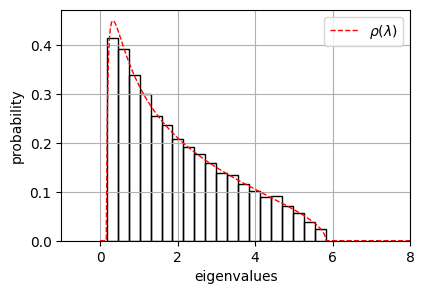
\includegraphics[width=\textwidth]{images/marchenko-pastur.white.png}
        \caption{Marchenko-Pastur law with $\phi = 2, n=2000, d=1000$ and $\rho(\lambda) = \frac{1}{\pi} \Im g(\lambda + i 0^+)$}
      \end{figure}
    \end{column}
  \end{columns}
  \begin{alertblock}{Conclusion \cite{belkin2020two,Hastie-Montanari-2019}}
  $$
  \Egen(r,\sigma,\phi,\lambda) = \sigma^2 + \lambda^2 r^2 g'(-\lambda) + \sigma^2 (g(-\lambda) - \lambda g'(-\lambda))
  $$
  \end{alertblock}
\end{frame}

\begin{frame}{Double-descent phenomenon}
  \begin{columns}
    \begin{column}{0.5\textwidth}
      %\vspace*{0.2cm}
      Take again the algebraic equations:
      \vspace*{-0.2cm}
      $$
      \begin{cases}
        -\lambda g^2 + (1 - \lambda - \phi) g +1 = 0 \\
        -\lambda (2gg' + g^2) + (1 - \lambda - \phi) g' + g = 0
      \end{cases}
      $$

      %\vspace*{0.1cm}

      Then in the limit $\lambda \to 0$:
      \begin{align*}
        \mathcal B_X(\hat \beta) & = \begin{cases} r^2 (1-\phi)  & \text{if } \phi < 1\\
        0 & \text{if } \phi > 1
        \end{cases}\\
        \mathcal V_X(\hat \beta) & = \begin{cases} \sigma^2 \frac{\phi}{1-\phi} & \text{if } \phi < 1\\
        \sigma^2 \frac{1}{\phi - 1} & \text{if } \phi > 1
        \end{cases}
      \end{align*}
    \end{column}
    \begin{column}{0.5\textwidth}
      % image marchenko-pastur.png with caption "\phi = 2"
      \vspace*{0.2cm}
      \begin{figure}
        \centering
        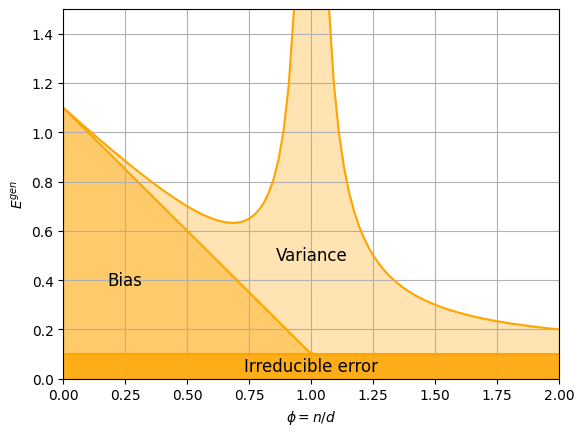
\includegraphics[width=\textwidth]{images/bias-variance.white.png}
        \caption{Test error $\sigma^2 = 0.1, r=1$}
      \end{figure}
    \end{column}
  \end{columns}

  \begin{alertblock}{Conclusion \cite{belkin2020two,Hastie-Montanari-2019}}
  \begin{equation*}
    \lim_{\lambda \to 0}\Egen(r,\sigma,\phi,\lambda) = \begin{cases}
      \sigma^2 + r^2 (1-\phi) + \sigma^2 \frac{ \phi}{1 - \phi} & \text{if } \phi < 1   \\
      \sigma^2 + \sigma^2 \frac{1}{\phi - 1} & \text{if } \phi > 1
  \end{cases}
  \end{equation*}
  \end{alertblock}
\end{frame}




\begin{frame}{More general models?}

  \emph{Marchenko-Pastur works well in that case, but what about more complex models?}

  \textbf{Non-exhaustive list of interesting models:}

  \begin{enumerate}
    \item Teacher-student model $Y = X \beta^*$ and $\hat Y = \hat X \beta$ with covariation structure $\Sigma = \mean[ x \hat x^T]$
    \item Random feature model: $\hat Y = \sigma(WX) \beta$ to have a notion of number of parameters
    \item Spike Wigner model: $Y = \beta^{*} \beta^{*T} + \xi$ 
    \item Matrix denoising: $Y = XX^T + \xi$
  \end{enumerate}

  \vspace*{0.3cm}

  \begin{block}{Is there a practical tool to analyze them?}
    \begin{center}
      \textbf{Linear-Pencils!}
    \end{center}
  \end{block}
\end{frame}

\section{Random matrix theory}

\begin{frame}{Level 1: Linear Pencil, the basics}

  Let $S$ be a symmetric random matrix ($S_{ij} \sim \mathcal N(0, \frac{1}{d})$) and define Stieltjes transform of the spectral density $\rho$ of $S$:
  $$ g(z) = \int \frac{\rho(\lambda) \dd \lambda}{\lambda - z} = \traceLim[d]{ (S - zI)^{-1}}$$

  \begin{block}{Main result \cite{wigner1958distribution}}
    \begin{equation}\label{eq:trivial-linear-pencil}
        g = (z-g)^{-1}
    \end{equation}
  \end{block}

  \textbf{Note 1:} above eqn. often represented under the form:
  $$g^2 - zg + 1 = 0$$

  \textbf{Note 2:} 
  $L=(S-zI)$ \emph{is} a "trivial" linear-pencil of size $1 \times 1$! 
  Equation \eqref{eq:trivial-linear-pencil} will follow us in the next slides.

\end{frame}


\begin{frame}{Level 2: the linearization method}
  Back to Marchenko-Pastur: $L = (X^TX - zI)$ is not a linear-pencil, because it is not "linear" in $X$.
  
  \textbf{But} we can linearize it with a block-matrix!

  Consider $U_1 = (X^TX - zI)^{-1}$ with:
  \begin{align*}
    \begin{cases}
      (X^TX - zI) U_1 & = I\\
      U_2 & = X U_1\\
    \end{cases}
  \end{align*}
  \vspace*{-0.1cm}
  Then we obtain our linear-pencil $L$:

  \begin{equation*}
    \underbrace{
    \begin{pmatrix}
      -zI & X^T\\
      X & -I
    \end{pmatrix}
    }_{L}
    \begin{pmatrix}
      U_1\\
      U_2
    \end{pmatrix}
    = \begin{pmatrix}
      I\\
      0
    \end{pmatrix}
  \end{equation*}
  And in particular, $\traceLim[d]{U_1}$ is given by the partial trace of $L^{-1}$ because:
  \begin{equation*}
    U_1 = \begin{pmatrix}
      I & 0
    \end{pmatrix}
    (L^{-1})
    \begin{pmatrix}
      I\\
      0
    \end{pmatrix}
    = (L^{-1})^{(11)}
  \end{equation*}
\end{frame}

\begin{frame}{Linear Pencil: the basics}
  \begin{columns}[T]
    \begin{column}{0.45\textwidth}
  \textbf{Step 1:} Encode matrix into a wider block-matrix (variance $\frac{1}{d}$):
  \begin{equation*}
    L = \begin{pmatrix}
      -z I_n & X\\
      X^T & -C^{-1}
    \end{pmatrix}
  \end{equation*}
\end{column}
\begin{column}{0.45\textwidth}

  \textbf{Step 2:} Extract deterministic blocks from random matrices:
  \begin{equation*}
    L_0 = \begin{pmatrix}
      -z I_n& 0\\
      0 & -C^{-1}
    \end{pmatrix}
  \end{equation*}
  \end{column}
  \end{columns}
    
  \textbf{Step 3:} Calculate block-wise covariance structure of $L$:
  $$
  \sigma_{12}^{21} = \sigma_{21}^{12} = 1 
  \qquad
  \qquad
  \sigma_{11}^{11} = \sigma_{22}^{22} = 0
  $$


  \textbf{Step 4:} Define the partial-trace of the inverse, and interesting operator:
  \begin{equation*}
    g_{ij} = \traceLim[d]{
      (L^{-1})^{(ij)}
    }
    \qquad \qquad
    [\eta_L(g)]_{il} = \sum_{jk \in \mathbb S} \sigma_{ij}^{kl} g_{jk}
  \end{equation*}

  \begin{block}{Main result \cite{spectra,mingo2017free}}
    \begin{equation}\label{eq:main-result-linear-pencil}
        g = \traceLimOp[d]{
            (L_0 - (\eta_L \otimes I)(g))^{-1}
        }
    \end{equation}
  \end{block}
\end{frame}

\begin{frame}{Linear Pencil: the basics}
  \begin{itemize}
    \item From \textbf{step 4} we have defined:
    \begin{equation}
      g_{11} = \traceLim[d]{ (XCX^T - zI_d)^{-1}}
    \end{equation}
    \item From application of \textbf{Main result} we find:
    \begin{equation*}
      \begin{pmatrix}
        g_{11} & 0\\
        0 & g_{22}
      \end{pmatrix}
      = \traceLimOp[d]{
        \begin{pmatrix}
          -zI_n - g_{22} I_n & 0\\
          0 & -C^{-1} - g_{11} I_d
        \end{pmatrix}^{-1}
      }
      \end{equation*}
  \end{itemize}



  \begin{alertblock}{Conclusion}
    With $g_C(z) = \traceLim[d]{ (C - zI_d)^{-1}}$:
    \begin{equation*}
      \begin{cases}
        g_{11} = \traceLim[d]{ (-zI_n - g_{22}I_n)^{-1} } = -\phi (z + g_{22})^{-1}\\
        g_{22} = \traceLim[d]{ (-C^{-1} - g_{11}I_d)^{-1} }
        = - g_{11}^{-1} \left( 
          1+ g_{11}^{-1} g_C(g_{11}^{-1})
          \right) 
      \end{cases}
    \end{equation*}
  \end{alertblock}

\end{frame}


\begin{frame}{Gaussian Equivalence Principle}
  How to calculate $g(z) = \traceLim[d]{(\sigma(WX) \sigma(WX)^T - zI_d)^{-1}}$?
  \begin{block}{GEP \cite{pennington2017nonlinear}}
    \begin{equation}
      \sigma(WX) \equiv
      \mu W X + \nu \Omega
    \end{equation}
    With:
    $
      0 = \langle \sigma, H_{e_0} \rangle
      \qquad
      \qquad
      \mu = \langle \sigma, H_{e_1} \rangle
      \qquad
      \qquad
      \mu^2 + \nu^2 = \langle \sigma, \sigma \rangle
    $
  \end{block}
  Ex.: $U = (\mu W, \nu \Omega), V^* = (X^T, I)$ so $g(z) = \traceLim[d]{(U V^T V U^T - zI_d)^{-1}}$
  \begin{equation*}
    L = \begin{pmatrix}
      -z I & 0 & 0 & U\\
      0 & 0 & V^T & I\\
      0 & V & I & 0\\
      U^T & I & 0 & 0
    \end{pmatrix}
    = \begin{pmatrix}
      -z I & 0 & 0 & 0 & \mu W & \nu \Omega\\
      0  & 0 & 0 & X & I & 0\\
      0  & 0 & 0& I & 0 & I\\
      0 & X^T & I & I & 0 & 0\\
      \mu W^T  & I & 0 & 0 & 0 & 0\\
      \nu \Omega^T & 0 & I & 0 & 0 & 0
    \end{pmatrix}
  \end{equation*}
  \textbf{Note:} no unique encoding! In fact, possible with a $4\times 4$ linear-pencil
\end{frame}

\section{The dynamics of general linear models}

\begin{frame}{Random Feature Model is just a structured linear model}
  \begin{block}{Gaussian covariate model \cite{loureiro2021capturing}}
    A mutual source of randomness $Z$, and two structures $A$ and $B$:
    \begin{equation*}
      Y = X \beta^* = (ZB) \beta^* \qquad \qquad \hat Y = \tilde X \beta = (Z A) \beta
    \end{equation*}
    With the generalization error:
    \begin{equation*}
      \Egen(\beta) = \mean \left[ ( x^T \beta^* - \tilde x^T \beta)^2 \right]
    \end{equation*}
  \end{block}

  \textbf{Ex.} Random feature model with $Z= (X_0 \quad \Omega \quad \xi)$ and:
  \begin{equation*}
    \beta^* = \begin{pmatrix}
      \beta_0^*\\
      1
    \end{pmatrix}
    \qquad
    B = \begin{pmatrix}
      I_d & O\\
      O & O\\
      0 & \sigma
    \end{pmatrix}
    \qquad
    A=\begin{pmatrix}
      \mu W \\
      \nu I_{N}\\
      0
    \end{pmatrix}
  \end{equation*}
  Then:
  \begin{equation*}
    Y = X_0 \beta_0^* + \xi \qquad \qquad \hat Y = \left( \mu W X_0 + \nu \Omega \right) \beta
    \equiv \sigma(WX_0) \beta
  \end{equation*}
\end{frame}

\begin{frame}{The dynamics of the Gaussian covariate model}
  \begin{block}{Main result \cite{bodin.2212.06757}}
    
  \resizebox{\textwidth}{!}{
    \begin{minipage}{1.3\textwidth}
      With gradient flow on: $\mathcal E_{\text{train}}^\lambda(\beta) = \frac{1}{n} \simplenorm{Y - \hat Y(\beta)}^2 + \frac{\lambda}{n} \norm{\beta}^2$
      \begin{equation*}
        \bar{\mathcal E}_{\text{gen}}(t) = c_0 + r_0^2 \mathcal B_0(t) + \mathcal B_1(t)
      \end{equation*}   
      With random initialization $\beta(t=0) \sim \mathcal N(0, r_0^2\frac{1}{d} I_{d})$ :
      \begin{align*}
        \mathcal B_1(t) & =
        \frac{-1}{4 \pi^2}
        \oint_\Gamma \oint_\Gamma
        \frac{
            (1-e^{-t(x+\lambda)})
            (1-e^{-t(y+\lambda)})
        }{
            (x + \lambda)(y + \lambda)
        } f_1(x,y) \dd x \dd y
         +
        \frac{1}{i \pi}
        \oint_\Gamma
        \frac{1-e^{-t(z+\lambda)}}{z + \lambda}
        f_2(z)
        \dd z\\
        \mathcal B_0(t) & =
        \frac{-1}{2i\pi}
        \oint_\Gamma
        e^{-2 t(z+\lambda)} f_0(z)
        \dd z
      \end{align*}
      And with $V=B \beta^{*} \beta^{*T} B^T$, $U = A A^T$, $c_0 = \traceLim[d]{V}$ and the self-consistent equations:
      \begin{align*}
        f_1(x,y) & = f_2(x) + f_2(y) + \tilde f_1(x,y) - c_0\\
        \tilde f_{1}(x,y) & = \traceLim[d]{
            (\phi U + \zeta_x I)^{-1} (\zeta_x \zeta_y V^* + \tilde f_{1}(x,y) \phi U^2 ) (\phi U + \zeta_y I)^{-1}
        }\\  
        f_2(z) & = c_0 - \traceLim[d]{\zeta_z V^* (\phi U + \zeta_z I)^{-1}}\\
        f_0(z) & = -\left(1+\frac{\zeta_z}{z}\right)\\
        \zeta_z & = -z + \traceLim[d]{ \zeta_z U (\phi U + \zeta_z I)^{-1}}
      \end{align*}    
    \end{minipage}
  }
\end{block}
\end{frame}

\begin{frame}{The limit $t\to+\infty$ of the Gaussian covariate model}
  \begin{block}{Secondary result \cite{bodin.2212.06757}}
    \begin{align*}
      \bar{\mathcal E}_{\text{gen}}(+ \infty) & = c_0 + f_1(-\lambda, -\lambda) + 2f_2(-\lambda) = \tilde f_1\\
      \bar{\mathcal E}_{\text{train}}^0 (+\infty) & = \lambda^2 \zeta^{-2} \bar{\mathcal E}_{\text{gen}}(+\infty)
    \end{align*}
    With $U_\star = \phi A^TA$ and $\Xi = \phi A^T B$ and:
    \begin{align*}
      f_1 & = 2 f_2 + \tilde f_1 - c_0\\
      f_1 & =  \traceLim[n]{ ( (\Xi \beta^* \beta^{*T} \Xi^T) + \tilde f_{1} U_\star ) U_\star (U_\star + \zeta I)^{-2}}\\
      f_2 & = \traceLim[n]{ (\Xi \beta^* \beta^{*T} \Xi^T) ( U_\star + \zeta I)^{-1}} \\
      \zeta & = \lambda + \traceLim[n]{ \zeta U_\star ( U_\star + \zeta I)^{-1}}
    \end{align*}
  \end{block}
  See also \cite{loureiro2021capturing}
\end{frame}

\begin{frame}{Example 1: Random feature - model/sample double-descents}

  \textbf{Ex.:} \href{http://127.0.0.1:8000/output.mp4}{Triple descent} \cite{dascoli2020triple, bodin2021model} 

  \vspace*{-0.2cm}
  \begin{figure}
    \centering
    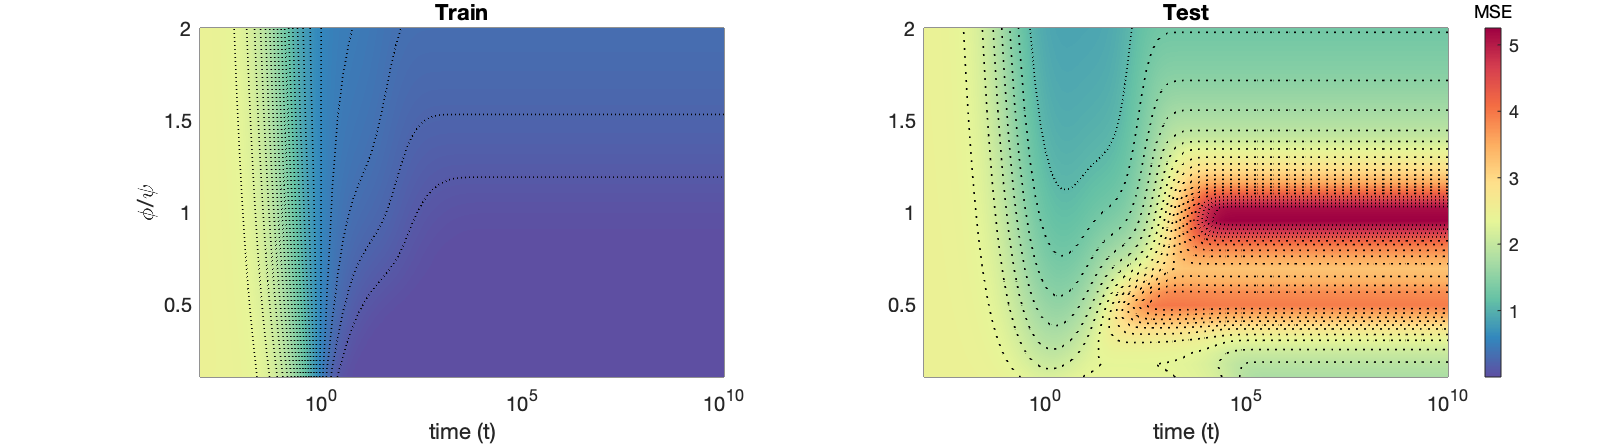
\includegraphics[width=\textwidth]{images/config4_2D.white.png}
    \caption{Parameters: $(\mu,\nu,\psi,r,s,\lambda) = (0.9,0.1,2,1,0.8,0.0001)$}
  \end{figure}
  \vspace*{-0.8cm}
  \begin{figure}[h!]
    \centering
    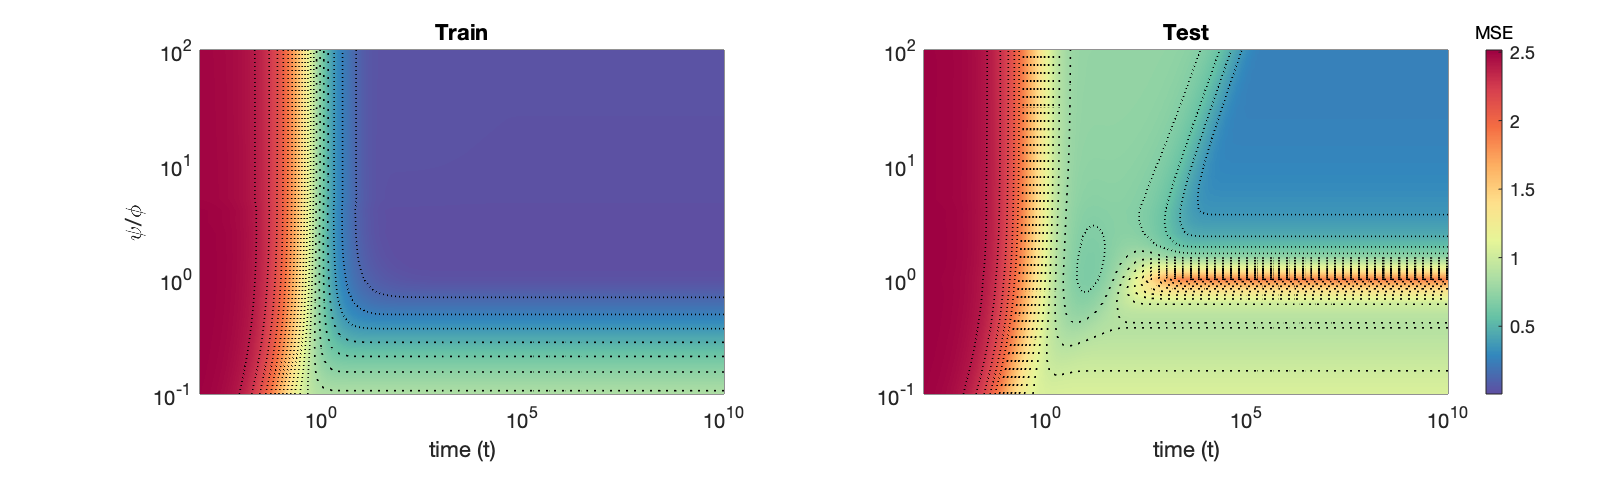
\includegraphics[width=1.0\textwidth]{images/config2_2D.white.png}
    \caption{Parameters $(\mu,\nu,\phi,r,s,\lambda) = (0.5,0.3,3,2.,0.4,0.001)$.
    }
  \end{figure}
\end{frame}

\begin{frame}{Example 2: Non-Isotropic regression - Descent structures}
  \vspace*{-0.5cm}
  \begin{equation*}
  B=I \quad \text{and} \quad A = \text{diag}(\underset{\frac{d}{p} \text{times}}{\underbrace{\alpha^{-\frac{0}{2}}, \ldots, \alpha^{-\frac{0}{2}}}}, 
  \underset{\frac{d}{p} \text{times}}{\underbrace{\alpha^{-\frac{1}{2}}, \ldots, \alpha^{-\frac{1}{2}}}}, \alpha^{-\frac{2}{2}}, \ldots, \alpha^{-\frac{p-1}{2}})
  \end{equation*}

  \vspace*{-0.5cm}
  \begin{columns}
    \begin{column}{0.5\textwidth}

    \begin{center}

      \begin{tikzpicture}
        \node[draw=none,shade,
            top color=grey,
            bottom color=grey,
            rounded corners=3pt,
            blur shadow={shadow blur steps=5}
        ] {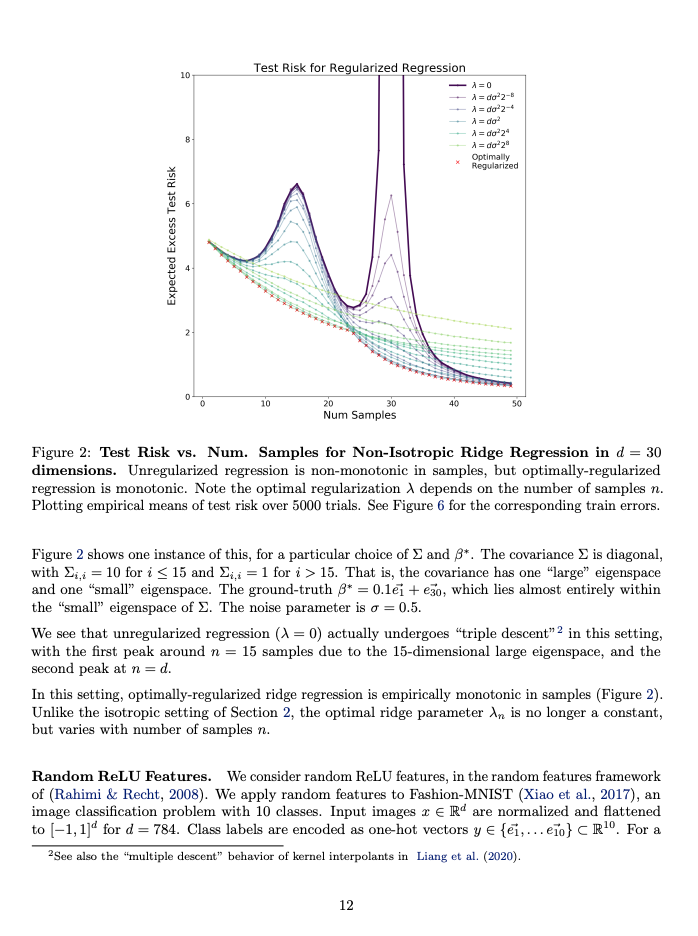
\includegraphics[width=0.5\textwidth]{images/paper-triple.png}};
      \end{tikzpicture}
      \cite{nakkiran2020optimal}
    \end{center}

    \end{column}
    \begin{column}{0.5\textwidth}
      \begin{figure}
        \centering
            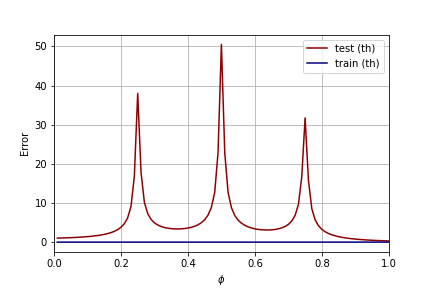
\includegraphics[width=\textwidth]{images/multiple-3descents.png}
        \caption{\footnotesize $p=4, \lambda=10^{-13}$, $\alpha = 10^4$
        }
      \end{figure}
    \end{column}
  \end{columns}


  \begin{block}{Result with $\alpha \to +\infty$ \cite{bodin.2212.06757}}
  \vspace*{-0.25cm}
    \begin{equation*}\footnotesize
      \bar{\mathcal E}_{\text{gen}}(+\infty) = \frac{1}{p} \sum_{k=0}^{p-1}
      \frac{\phi (1-\phi)}{
          \left( \phi - \frac{k}{p} \right) \left( \frac{k + 1}{p} - \phi \right) 
      }  \mathds{1}_{\left] \frac{k}{p}; \frac{k+1}{p} \right[}(\phi) - \phi + o_\alpha(1)
  \end{equation*}
  \vspace*{-0.25cm}
  \end{block}

\end{frame}


\begin{frame}{Example 3: Realistic datasets} 
  \begin{itemize}
    \item \textbf{Data:} MNIST dataset $X_0 \in \mathbb R^{n_{tot} \times d}$ with normalized entries and $n_{tot}=60'000$ and $d=28\times 28 = 784$
    \item \textbf{Aim:} Learning the parity ($y=\pm1$ for even/odd numbers)
    \item \textbf{Structure:} cov. matrix $U_\star \simeq \frac{1}{n_{tot}} X^TX$ and $\Xi \beta^* \simeq X^TY$ (since $X^TX = A^T (Z^T Z) A$ and $X^T Y = A (Z^T Z) B \beta^*$ and $n_{tot} \gg d$)
  \end{itemize}
  \vspace*{-0.7cm}
  \begin{figure}
    \centering
    \subfloat{
        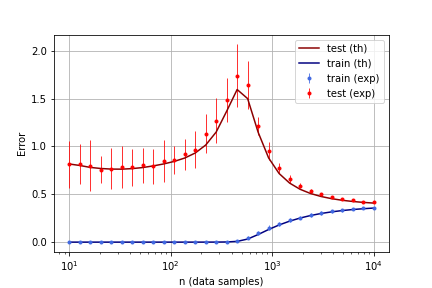
\includegraphics[width=0.5\textwidth]{images/lsq_profile.png}
    }
    \subfloat{
        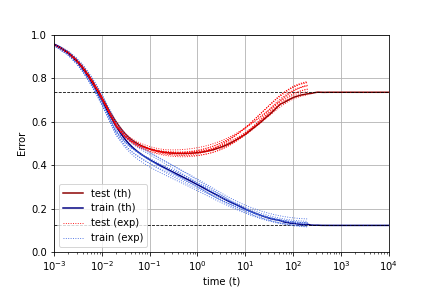
\includegraphics[width=0.5\textwidth]{images/evolution1.png}
    }
    \caption{\footnotesize 
        Comparison between the analytical and experimental learning profiles for the minimum least-squares estimator at $\lambda = 10^{-3}$ on the left (20 runs) and the time evolution at $\lambda = 10^{-2}, n=700$ on the right (10 runs).
    }
  \end{figure}
\end{frame}

\section{Beyond the linear setting}


\begin{frame}{Spiked Wigner Model}
  \begin{itemize}
    \item \textbf{The data:} $ Y = \theta^* \theta^{*T} + \sqrt{\frac{n}{\lambda}} \xi$ with $\xi_{ij} \sim \mathcal N(0, 1)$ and $\norm{\theta^*}^2 = n$.
    \item \textbf{The objective:} Minimizing $\mathcal H(\theta) = \norm{Y-\theta \theta^T}_F^2$.
  \end{itemize}
  \emph{Equivalently: maximizing $\theta^T Y \theta$ subject to $\norm{\theta}^2 = n$, ie. top eigenvector}
  \begin{figure}[H]
      \centering
      \subfloat{
          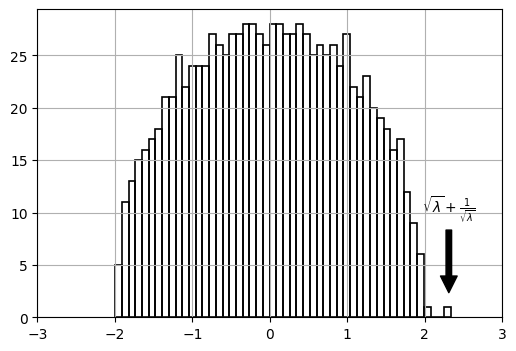
\includegraphics[width=0.5\textwidth]{images/eigenvalue-outlier.white.png}
      }
      \subfloat{
          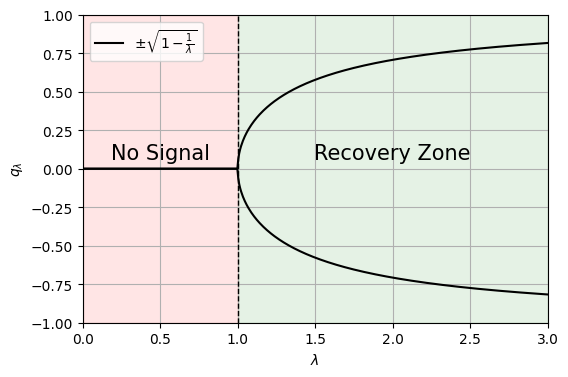
\includegraphics[width=0.5\textwidth]{images/bbp-transition2.white.png}
      }
      \caption{Histogram of the eigenvalues of $Y$ (left) and the theoretical transition of the overlap in the high-dimensional limit (right).}
  \end{figure}
  
  \vspace*{-0.25cm}
  \textbf{Metric:} overlap $q(\theta)$ with: $\frac{1}{n} \norm{\theta^* - \theta}_F^2 = 2(1 - \theta^T \theta^* ) = 2 (1 - q(\theta))$

\end{frame}

\begin{frame}{Main result: gradient-flow evolution}
  Random initialization $\theta_0\in \mathbb{S}^{n-1}(\sqrt  n)$ and gradient flow method
  \begin{equation*}
    \frac{\dd \theta_t}{\dd t} = - \nabla \mathcal H(\theta_t)
    + \frac{1}{n} \left( \theta_t^T \nabla \mathcal H(\theta_t)  \right) \theta_t  
  \end{equation*}

  \begin{block}{Theorem \cite{pmlr-v134-bodin21a}}
      With $q(0) = \frac{1}{n} \langle\theta^*, \theta_{0}\rangle = \alpha$ for a fixed $\alpha \in [-1, +1]$:
      \begin{equation*}
      q(\tau) \overset{\mathbb{P}}{ \underset{n \to\infty}{\longrightarrow}} \bar q(\tau) = \frac{\hat q(\tau)}{\sqrt{\hat p(\tau)}}
      \end{equation*}
      where\footnote{$M_\lambda(\tau) = \frac{\sqrt\lambda}{\tau} I_1(\frac{2\tau}{\sqrt{\lambda}})$ scaled moment generating function of semicircle law} 

  \vspace*{-0.25cm}
  \resizebox{\textwidth}{!}{
    \begin{minipage}{1.3\textwidth}
      \begin{align*}
      \hat q(\tau) & = 
      \alpha e^{(1+\frac{1}{\lambda}) \tau} 
      \left\{ 1 - \frac{1}{\lambda} \int_0^\tau ds\, e^{-(1+\frac{1}{\lambda}) s} M_\lambda(s) \right\} \\
      \hat p(\tau) & = M_\lambda(2\tau) + 2 \alpha \int_0^\tau ds\, \hat q(s) M_\lambda(2\tau-s)
              + \int_0^\tau\int_0^\tau dudv\, \hat q(u) \hat q(v) M_\lambda(2\tau-u-v).
      \end{align*}
      \end{minipage}
  }
  \end{block}
  \vspace*{0.5cm}
\end{frame}


\begin{frame}{Integro-differential equations}
  Let's define \emph{state evolution functions} with resolvent $\mathcal R(z) = (\frac{\xi}{\sqrt n} - z I)^{-1}$
  $$Q_t(z) = \frac{1}{n} \langle \theta^*, \mathcal R(z) \theta_t \rangle, ~~~~ 
  P_t(z) = \frac{1}{n} \langle \theta_t, \mathcal R(z) \theta_t \rangle, ~~~~ 
  R(z) = \frac{1}{n} \langle \theta^*, \mathcal R(z) \theta^* \rangle$$
  $\Rightarrow$ Closed set of integro-differential-equations:
  \begin{align*}
      \begin{cases}
          \frac{\dd}{\dd t}Q_t(z) = q(t) R(z) 
                                     + \frac{1}{\sqrt \lambda} (z Q_t(z) + q(t))
                                      - \left(q^2(t) + \frac{1}{\sqrt \lambda} p_1(t) \right) Q_t(z) 
          \\
          \frac12 \frac{\dd}{\dd t} P_t(z) = q(t) Q_t(z) 
                                              + \frac{1}{\sqrt \lambda} (z P_t(z) + 1)
                                               - \left(q^2(t) + \frac{1}{\sqrt \lambda} p_1(t) \right) P_t(z)
      \end{cases}
  \end{align*}

  \begin{columns}
    \begin{column}{0.5\textwidth}
      with:
      \begin{equation*}
        \begin{cases}
          q(t) = \oint_{\mathcal C} \frac{-\dd z}{2i \pi} Q_t(z)\\
          p_1(t) = \oint_{\mathcal C} \frac{-\dd z}{2i \pi} z P_t(z) = \frac{1}{n} \theta_t^T \frac{\xi}{\sqrt n} \theta_t     
        \end{cases}
      \end{equation*}
    
    \end{column}
    \begin{column}{0.5\textwidth}
      \begin{figure}
        \centering
          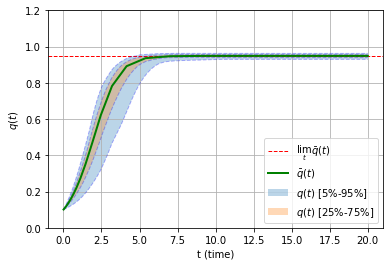
\includegraphics[width=0.8\textwidth]{images/run_1.png}
        \caption{$\lambda = 10, \alpha = 0.1, n=70$}
    \end{figure}
    \end{column}
  \end{columns}
\end{frame}


\begin{frame}{Integro-differential equations}
  \begin{enumerate}
      \item Simplify the system using a \emph{change of variable} such as:
      \begin{equation}
          \hat Q_t(z) = e^{\int_0^t q^2(s) + \frac{1}{\sqrt \lambda} p_1(s) \dd s} Q_t(z)
      \end{equation}
      \item \emph{Laplace transform} introduces the initial conditions $Q_0(z), P_0(z)$
      \item Convergence in probability (and uniformly in $z$ on a fixed contour) of the initial conditions towards the Stieltjes transform of the semicircle law $G_{\rm sc}(z) = \frac12(-z + \sqrt{z^2 - 4})$ for any deterministic $\theta_0, \theta^*$ such that $\alpha = q(0)$ for a fixed $\alpha > 0$ :
      \begin{equation}
          (Q_0(z), P_0(z), R(z)) \to (\alpha G_{\rm sc}(z), G_{\rm sc}(z), G_{\rm sc}(z))
      \end{equation}
      \item \emph{Cauchy Integration} to isolate the terms $\mathcal L \hat q(t), \mathcal L \hat p(t)$ 
      \item \emph{Inverse laplace transform} of the former terms and calculation of the ideal solution of the system with the limiting initial conditions
      \item Grönwall-type arguments to show the concentration towards the calculated ideal-solution
  \end{enumerate}
\end{frame}



\begin{frame}{First order asymptotics}
  \begin{block}{Result $\tau \to +\infty$:}
    \resizebox{\textwidth}{!}{
      \begin{minipage}{1.3\textwidth}
    \begin{itemize}
      \item For $1 < \lambda < +\infty$:
      \vspace{-0.2cm}
      \begin{equation*}
          \bar q(\tau) - \text{sign}(\alpha) \sqrt{1-\frac{1}{\lambda}}
          \sim\frac{  \text{sign}(\alpha)  
              }{2 \sqrt{\pi} \lambda^\frac14 \sqrt{1-\frac{1}{\lambda}}  \left(1 - \frac{1}{\sqrt{\lambda}}\right)^2}  
              \tau^{-\frac32}  e^{ -(1-\frac{1}{\sqrt \lambda})^2 \tau } 
      \end{equation*}
      \item For $0 < \lambda < 1$:
      \vspace{-0.2cm}
      \begin{equation*}
        \bar q(\tau)
        \sim  
        \frac{ \alpha \left( \frac{2}{\pi} \right)^\frac14  }{
            \lambda^\frac58 
            \left(1 - \frac{1}{\sqrt{\lambda}}\right)^2
            \sqrt{
            1 - \alpha^2 + \frac{\alpha^2}{\lambda (\frac{1}{\sqrt \lambda} - 1)^2 }
        }} \tau^{- \frac34}
      \end{equation*}
    \end{itemize}
    \vspace{-0.2cm}
    \end{minipage}
    }
  \end{block}
  \begin{figure}
    \centering
    \begin{subfigure}{0.48\linewidth}
        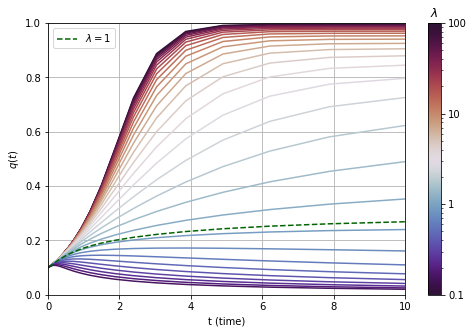
\includegraphics[width=\textwidth]{./images/experiment_2.png} 
        \caption{$\alpha = 0.1$}
    \end{subfigure}
    \hfill
    \begin{subfigure}{0.48\linewidth}
        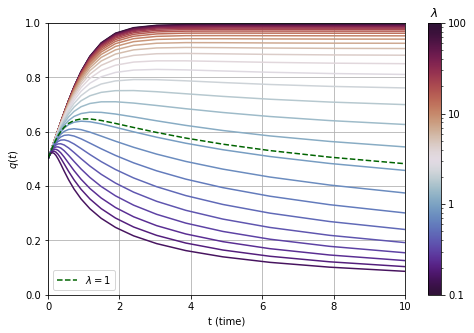
\includegraphics[width=\textwidth]{./images/experiment_3.png}
        \caption{$\alpha = 0.5$}
    \end{subfigure}
    \caption{Overlap as a function of time according to theorem \ref{th:risktrack} for two initial conditions and different 
    signal-to-noise ratios. Thick dotted line corresponds to $\lambda =1$ and tends to zero slowly as $(2/\pi\tau)^{1/4}$. For $\lambda <1$ the curves tend to zero and for $\lambda >1$ they tend to $\sqrt{1 - 1/\lambda}$. }
    \label{fig:theoretical_curves}
\end{figure}
\end{frame}


\begin{frame}{Quick overview: Extensive case}
  \begin{itemize}
    \item \textbf{The data:} $ Y = X^* X^{*T} + \frac{1}{\sqrt \lambda} \xi$ with $\xi_{ij},X_{ij}^*  \sim \mathcal N(0,\frac{1}{n})$ 
    \item \textbf{The objective:} Minimizing\footnote{See also Rotationally Invariant Estimator \cite{potters2020first}}
    $\mathcal H(X) = \norm{Y-XX^T}^2_F$ with $X \in \mathbb R^{n \times m}$.
  \end{itemize}

  Gradient-flow equation $\frac{\dd X_t}{\dd t} = - \phi \nabla \mathcal H(X_t)$ is a matrix Riccati differential equation with solution:

    \begin{equation*}
      X_t X_t^T = e^{tY} \textcolor{red}{X_0} \left( 
        I + 2 \textcolor{red}{X_0^T} \int_0^t e^{2sY} \dd s \textcolor{red}{X_0}
        \right)^{-1} \textcolor{red}{X_0^T} e^{tY}
    \end{equation*}

    \textbf{Metric:} $\mathcal E(X) = \lim_{d} \frac{1}{d} \mean \norm{X^* X^{*T} - XX^T}_F^2 = \text{cst} - 2 q_t + p_t$ with:
    \begin{equation*}
      q_t = \traceLim[d]{(X^*X^{*T}) (X_t X_t^T)}
      \qquad
      p_t = \traceLim[d]{(X_t X_t^T)^2}
    \end{equation*}

\end{frame}

\begin{frame}{Overlap Solution}
  With $L_t = 2\int_0^t e^{2sY}\dd s$ and linear-pencil method:
  \begin{equation*}
    \begin{cases}
      g_{11} &= \traceLim[d]{ g_{44} \psi X^* e^{tY} ( g_{44} \psi L_t + I_n)^{-1} e^{tY} X^{*T} } \\
      g_{44} & = (1-g_{66})^{-1} \\
      g_{66} &= -\traceLim[n]{ L_t (g_{44} \psi L_t + I_n)^{-1}  }
    \end{cases}
  \end{equation*}
  \begin{block}{Main result \cite{bodin10161669}}
    \begin{equation*}
        q_t = \int_{\mathbb R} 
        \frac{z \rho_Q(z) \dd z}{
            1 - e^{-2tz} + z \textcolor{red}{\tilde q_t} e^{-2tz}
        }
    \end{equation*}
    With $g_Q(z) = \traceLim[d]{X^{*T} (Y-zI)^{-1} X^*}$ and $g_P(z) = \traceLim[d]{(Y-zI)^{-1}}$
    \begin{equation*}
        \psi \textcolor{red}{\tilde q_t} = 1 + \int_{\mathbb R}  \frac{
            (1- e^{-2tz}) \rho_P(z) \dd z
        }{
            \frac{1}{\tilde q_t} (1 - e^{-2tz}) + z e^{-2tz}
        }
    \end{equation*}
  \end{block}

\end{frame}

\section{Conclusion}

\begin{frame}{Learning the first layer}
  \begin{columns}[T]
    \begin{column}{0.5\textwidth}
        \begin{block}{}
          \textbf{Gradient-flow} \cite{NEURIPS2022_f7e7fabd}
          \begin{equation*}
            \frac{\dd W_t}{\dd t} = X^T \left[ (
                Y - \hat Y
              ) \beta_t^T  \odot \sigma'(XW_t)
            \right]
          \end{equation*}

          Rank-one update emerge with one-gradient step and specific scalings of $\beta_0$
        \end{block}

        \begin{block}{}
          \textbf{Mean-field view} \cite{mei2018mean}
          centered isotropic gaussian model:
          \begin{equation*}
            \partial_t \rho(r,t) =
            2\xi(t) \partial_r ( \rho(r,t) \partial_r \psi(r, \rho))
          \end{equation*}

          (with $r=\norm{w}_2$)
        \end{block}
    \end{column}
    \begin{column}{0.54\textwidth}
      \begin{block}{}
        \textbf{Low-rank adaptation} \cite{hu2021lora}\\
        Train only a low-rank matrix
        \vspace*{-0.3cm}
        \begin{figure}
          \centering
          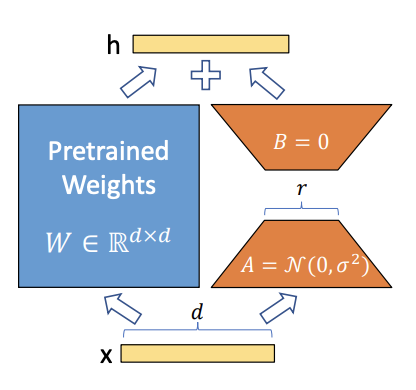
\includegraphics[width=0.8\textwidth]{images/lora.white.png}
          \vspace*{-0.3cm}
          \caption{LoRA (Extracted from above reference)}
        \end{figure}
      \end{block}
    \end{column}
  \end{columns}

\end{frame}

\begin{frame}{Empirical scaling laws}
  \cite{kaplan2020scaling} \emph{(OpenAI)} used for GPT3, further challenged in secondary paper \cite{hoffmann2022training} \emph{(Deepmind)}, but common observation:

  \begin{center}
    \emph{"the training curves follow predictable power-laws [...]"}
  \end{center}  

  \textbf{Example:} loss $L$, computational resources $C$,  model size $N$, available data $D$:
  \begin{align*}
    L & = A N^{-\alpha} + B D^{-\beta} + L_0\\
    C & = C_0 N D
  \end{align*}
  
  \begin{alertblock}{Final Question:}
    Can we derive scaling laws from first principle?
  \end{alertblock}
\end{frame}


\begin{frame}[standout]
  Questions?
\end{frame}

\begin{frame}{Appendix: Construction of $4\times 4$ linear pencil}
  Consider $\traceLim[d]{(\sigma(XW) \sigma(XW)^{T} - zI)^{-1}} = \traceLim[d]{U_0}$:
  \begin{align*}
    ((\mu W X + \nu \Omega) (\mu X^T W^T + \nu \Omega^T) - z I) U_0 & = I\\
    U_1 & = \mu W^T U_0 \\
    U_2 & = X^T U_1 + \nu \Omega^T U_0\\
    U_3 & = X U_2
  \end{align*}
  So first equation is: $ \mu W U_3 + \nu \Omega U_2 - z U_0 = I$, so:
  \begin{align*}
    \begin{pmatrix}
      -z I & 0 & \nu \Omega & \mu W\\
      0 & 0 & X & -I\\
      \nu \Omega^T & X^T & -I & 0\\
      \mu W^T & -I & 0 & 0
    \end{pmatrix}
    \begin{pmatrix}
      U_0\\
      U_1\\
      U_2\\
      U_3
    \end{pmatrix}
    = 
    \begin{pmatrix}
      I\\
      0\\
      0\\
      0
    \end{pmatrix}
  \end{align*}

\end{frame}


\begin{frame}{Appendix: Gaussian Equivalence Principle}
  From \cite{lu2022equivalence,mei2020generalization} with $y,x \in \mathbb S^{d-1}$ , decomposition with Gegenbauer polynomials:
  \begin{equation*}
    \sigma(\sqrt{d} x^T y) = \sum_{k=1}^{p} \alpha_k q_k(\sqrt{d} x^T y)
  \end{equation*}
  (In high-dimenion, $\alpha_k$ are related to the coefficients of the Hermite polynomials decomposition).\\
  Decoupling with spherical harmonics $Y_{k,a}$:
  \begin{equation*}
    q_k(\sqrt{d} x^T y) = \frac{1}{\sqrt{N_k}} \sum_{a=0}^{N_k} Y_{k,a}(x) Y_{k,a}(y)
  \end{equation*}
\end{frame}
  


\begin{frame}{Appendix: Bias-variance decomposition}
  Classical bias-variance decomposition over new data point $x$:
  \begin{align}
    \mean[(y - \hat y )^2] & = \mean[y - \hat y]^2 + \var(\hat y) + \var(y)
  \end{align}
  Is true when:
  \begin{align}
    \var(y - \hat y) = \var(\hat y) + \var(y)
    \implies \cov(y, \hat y)=0
  \end{align}
  This is true for the R.V. $\beta_0, \xi, X, \epsilon$ (because each of them only affect either $y$ and $\hat y$) but not for $x$ (and $\beta^*$ if considered random). So in fact we implicitly always require the conditional expectation on $x$:
  \begin{align}
    \mean[(y - \hat y )^2] & = \mean_x\left[ \mean[y - \hat y| x]\right]^2 + \mean_x \var(\hat y | x) + \mean_x \var(y | x)
  \end{align}
\end{frame}



\begin{frame}{From statistical physics to machine learning}
  \begin{columns}
    \begin{column}{0.5\textwidth}
        \begin{center}
          Study of large systems of \\
          \emph{interacting particles}\\
            or\\
          \emph{interacting parameters}
        \end{center}
    
      \begin{block}{Common points}
        \begin{itemize}
          \item \textbf{Randomness:} initialization, noise, data
          \item \textbf{High-dimensional limit}
          \item \textbf{Phase transitions:} sharp changes in the behavior of the system
          \item \textbf{Methods:} replica method, RMT, cavity method
        \end{itemize}
      \end{block}
    \end{column}
    \begin{column}{0.5\textwidth}
      \textbf{Ex.:} Hopfield Network \cite{hopfield1982neural}
      \begin{center}
        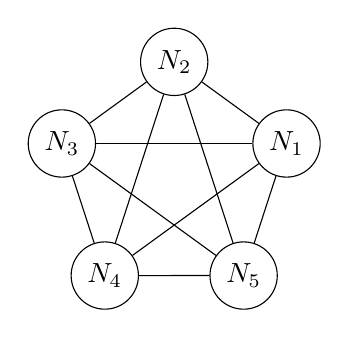
\begin{tikzpicture}[scale=1.5]
          \foreach \i in {1,...,5} {
              \node[draw,circle] (N\i) at ({360/5*(\i-1)+360/20}:1) {$N_{\i}$};
          }
          \foreach \i in {1,...,5} {
              \foreach \j in {\i,...,5} {
                  \draw (N\i) -- (N\j);
              }
          }
          \end{tikzpicture}
      \end{center}
      \begin{equation*}
        E = -\frac12\sum_{i,j} w_{ij} S_i S_j -\sum_i \theta_i S_i
      \end{equation*}
    \end{column}
  \end{columns}

\end{frame}

\appendix

\begin{frame}[allowframebreaks, noframenumbering]{References}

  \bibliographystyle{apalike}
  \bibliography{bibliography}

\end{frame}

\end{document}
